% Generated by make_figures.py; edit that script instead of this file.
\documentclass[tikz,border=7pt]{standalone}
\usepackage{amsmath}
\usetikzlibrary{arrows.meta,calc,positioning,decorations.pathreplacing}
\def\figcellw{0.62cm}\def\figcellh{0.32cm}
% Shared palette and TikZ styles for the information-flow figures.
%
% Each figure sets its cell size before loading this file:
%   \def\figcellw{0.80cm}\def\figcellh{0.36cm}
%   % Shared palette and TikZ styles for the information-flow figures.
%
% Each figure sets its cell size before loading this file:
%   \def\figcellw{0.80cm}\def\figcellh{0.36cm}
%   % Shared palette and TikZ styles for the information-flow figures.
%
% Each figure sets its cell size before loading this file:
%   \def\figcellw{0.80cm}\def\figcellh{0.36cm}
%   \input{figure_style}
\providecommand{\figcellw}{0.80cm}
\providecommand{\figcellh}{0.36cm}

% ------------------------------------------------------------
% Palette
% ------------------------------------------------------------
\definecolor{frameblue}{RGB}{42,66,167}
\definecolor{headerfill}{RGB}{238,242,252}
\definecolor{activefill}{RGB}{210,235,250}
\definecolor{activedraw}{RGB}{0,137,225}
\definecolor{ghostfill}{RGB}{222,228,236}
\definecolor{ghostdraw}{RGB}{145,154,168}
\definecolor{depthfill}{RGB}{249,221,187}
\definecolor{depthdraw}{RGB}{216,108,19}
\definecolor{tempfill}{RGB}{229,210,252}
\definecolor{tempdraw}{RGB}{119,45,205}

% ------------------------------------------------------------
% Styles
% ------------------------------------------------------------
\tikzset{
  % Frames and headers
  panel/.style={draw=frameblue, rounded corners=4pt, line width=0.9pt},
  header/.style={draw=frameblue, fill=headerfill, rounded corners=4pt, line width=0.9pt},
  sideheader/.style={header},
  descbox/.style={draw=frameblue!55, fill=white, rounded corners=2.5pt, line width=0.6pt,
    inner sep=2pt, align=center, font=\footnotesize,
    execute at begin node={\hyphenpenalty=10000\exhyphenpenalty=10000\relax}},
  divider/.style={draw=frameblue, dashed, line width=0.8pt},
  % Layer and block cells
  cell/.style={rounded corners=2pt, minimum width=\figcellw, minimum height=\figcellh, inner sep=0pt},
  active/.style={cell, draw=activedraw, fill=activefill, line width=0.82pt},
  ghost/.style={cell, draw=ghostdraw, fill=ghostfill, fill opacity=0.42, draw opacity=0.58, line width=0.72pt},
  depthmark/.style={cell, draw=depthdraw, fill=depthfill, line width=0.95pt},
  tempmark/.style={cell, draw=tempdraw, fill=tempfill, line width=0.95pt},
  depthcell/.style={depthmark},
  tempcell/.style={tempmark},
  ghostdepth/.style={cell, draw=depthdraw, fill=depthfill, fill opacity=0.28, draw opacity=0.55, line width=0.90pt},
  ghosttemp/.style={cell, draw=tempdraw, fill=tempfill, fill opacity=0.28, draw opacity=0.55, line width=0.90pt},
  notrun/.style={cell, draw=ghostdraw, dashed, draw opacity=0.7, line width=0.6pt},
  stateT/.style={cell, draw=tempdraw, fill=tempfill, inner sep=1pt, line width=0.9pt, font=\footnotesize},
  stateD/.style={cell, draw=depthdraw, fill=depthfill, inner sep=1pt, line width=0.9pt, font=\footnotesize},
  % State injection points
  injectD/.style={circle, draw=depthdraw, fill=depthfill, minimum size=3.6mm,
    inner sep=0pt, line width=0.85pt, font=\bfseries\scriptsize},
  injectT/.style={circle, draw=tempdraw, fill=tempfill, minimum size=3.6mm,
    inner sep=0pt, line width=0.85pt, font=\bfseries\scriptsize},
  % Arrows
  flow/.style={-{Latex[length=1.8mm]}, draw=black, line width=0.82pt},
  injflow/.style={-{Latex[length=1.25mm]}, draw=black, line width=0.82pt},
  ghostflow/.style={-{Latex[length=1.5mm]}, draw=black!38, line width=0.58pt},
  dread/.style={-{Latex[length=1.9mm]}, draw=depthdraw, dashed, line width=0.95pt},
  tread/.style={-{Latex[length=1.9mm]}, draw=tempdraw, dashed, line width=0.95pt},
  % Labels
  brace label/.style={midway, xshift=-0.86cm, align=right, text width=1.32cm, font=\footnotesize},
  rlabel/.style={anchor=east, font=\footnotesize, align=right, text width=1.65cm},
  stage/.style={anchor=east, font=\footnotesize, align=right, text width=1.8cm},
  tinylabel/.style={font=\footnotesize, align=center},
  legendtext/.style={anchor=west, font=\footnotesize},
}

\providecommand{\figcellw}{0.80cm}
\providecommand{\figcellh}{0.36cm}

% ------------------------------------------------------------
% Palette
% ------------------------------------------------------------
\definecolor{frameblue}{RGB}{42,66,167}
\definecolor{headerfill}{RGB}{238,242,252}
\definecolor{activefill}{RGB}{210,235,250}
\definecolor{activedraw}{RGB}{0,137,225}
\definecolor{ghostfill}{RGB}{222,228,236}
\definecolor{ghostdraw}{RGB}{145,154,168}
\definecolor{depthfill}{RGB}{249,221,187}
\definecolor{depthdraw}{RGB}{216,108,19}
\definecolor{tempfill}{RGB}{229,210,252}
\definecolor{tempdraw}{RGB}{119,45,205}

% ------------------------------------------------------------
% Styles
% ------------------------------------------------------------
\tikzset{
  % Frames and headers
  panel/.style={draw=frameblue, rounded corners=4pt, line width=0.9pt},
  header/.style={draw=frameblue, fill=headerfill, rounded corners=4pt, line width=0.9pt},
  sideheader/.style={header},
  descbox/.style={draw=frameblue!55, fill=white, rounded corners=2.5pt, line width=0.6pt,
    inner sep=2pt, align=center, font=\footnotesize,
    execute at begin node={\hyphenpenalty=10000\exhyphenpenalty=10000\relax}},
  divider/.style={draw=frameblue, dashed, line width=0.8pt},
  % Layer and block cells
  cell/.style={rounded corners=2pt, minimum width=\figcellw, minimum height=\figcellh, inner sep=0pt},
  active/.style={cell, draw=activedraw, fill=activefill, line width=0.82pt},
  ghost/.style={cell, draw=ghostdraw, fill=ghostfill, fill opacity=0.42, draw opacity=0.58, line width=0.72pt},
  depthmark/.style={cell, draw=depthdraw, fill=depthfill, line width=0.95pt},
  tempmark/.style={cell, draw=tempdraw, fill=tempfill, line width=0.95pt},
  depthcell/.style={depthmark},
  tempcell/.style={tempmark},
  ghostdepth/.style={cell, draw=depthdraw, fill=depthfill, fill opacity=0.28, draw opacity=0.55, line width=0.90pt},
  ghosttemp/.style={cell, draw=tempdraw, fill=tempfill, fill opacity=0.28, draw opacity=0.55, line width=0.90pt},
  notrun/.style={cell, draw=ghostdraw, dashed, draw opacity=0.7, line width=0.6pt},
  stateT/.style={cell, draw=tempdraw, fill=tempfill, inner sep=1pt, line width=0.9pt, font=\footnotesize},
  stateD/.style={cell, draw=depthdraw, fill=depthfill, inner sep=1pt, line width=0.9pt, font=\footnotesize},
  % State injection points
  injectD/.style={circle, draw=depthdraw, fill=depthfill, minimum size=3.6mm,
    inner sep=0pt, line width=0.85pt, font=\bfseries\scriptsize},
  injectT/.style={circle, draw=tempdraw, fill=tempfill, minimum size=3.6mm,
    inner sep=0pt, line width=0.85pt, font=\bfseries\scriptsize},
  % Arrows
  flow/.style={-{Latex[length=1.8mm]}, draw=black, line width=0.82pt},
  injflow/.style={-{Latex[length=1.25mm]}, draw=black, line width=0.82pt},
  ghostflow/.style={-{Latex[length=1.5mm]}, draw=black!38, line width=0.58pt},
  dread/.style={-{Latex[length=1.9mm]}, draw=depthdraw, dashed, line width=0.95pt},
  tread/.style={-{Latex[length=1.9mm]}, draw=tempdraw, dashed, line width=0.95pt},
  % Labels
  brace label/.style={midway, xshift=-0.86cm, align=right, text width=1.32cm, font=\footnotesize},
  rlabel/.style={anchor=east, font=\footnotesize, align=right, text width=1.65cm},
  stage/.style={anchor=east, font=\footnotesize, align=right, text width=1.8cm},
  tinylabel/.style={font=\footnotesize, align=center},
  legendtext/.style={anchor=west, font=\footnotesize},
}

\providecommand{\figcellw}{0.80cm}
\providecommand{\figcellh}{0.36cm}

% ------------------------------------------------------------
% Palette
% ------------------------------------------------------------
\definecolor{frameblue}{RGB}{42,66,167}
\definecolor{headerfill}{RGB}{238,242,252}
\definecolor{activefill}{RGB}{210,235,250}
\definecolor{activedraw}{RGB}{0,137,225}
\definecolor{ghostfill}{RGB}{222,228,236}
\definecolor{ghostdraw}{RGB}{145,154,168}
\definecolor{depthfill}{RGB}{249,221,187}
\definecolor{depthdraw}{RGB}{216,108,19}
\definecolor{tempfill}{RGB}{229,210,252}
\definecolor{tempdraw}{RGB}{119,45,205}

% ------------------------------------------------------------
% Styles
% ------------------------------------------------------------
\tikzset{
  % Frames and headers
  panel/.style={draw=frameblue, rounded corners=4pt, line width=0.9pt},
  header/.style={draw=frameblue, fill=headerfill, rounded corners=4pt, line width=0.9pt},
  sideheader/.style={header},
  descbox/.style={draw=frameblue!55, fill=white, rounded corners=2.5pt, line width=0.6pt,
    inner sep=2pt, align=center, font=\footnotesize,
    execute at begin node={\hyphenpenalty=10000\exhyphenpenalty=10000\relax}},
  divider/.style={draw=frameblue, dashed, line width=0.8pt},
  % Layer and block cells
  cell/.style={rounded corners=2pt, minimum width=\figcellw, minimum height=\figcellh, inner sep=0pt},
  active/.style={cell, draw=activedraw, fill=activefill, line width=0.82pt},
  ghost/.style={cell, draw=ghostdraw, fill=ghostfill, fill opacity=0.42, draw opacity=0.58, line width=0.72pt},
  depthmark/.style={cell, draw=depthdraw, fill=depthfill, line width=0.95pt},
  tempmark/.style={cell, draw=tempdraw, fill=tempfill, line width=0.95pt},
  depthcell/.style={depthmark},
  tempcell/.style={tempmark},
  ghostdepth/.style={cell, draw=depthdraw, fill=depthfill, fill opacity=0.28, draw opacity=0.55, line width=0.90pt},
  ghosttemp/.style={cell, draw=tempdraw, fill=tempfill, fill opacity=0.28, draw opacity=0.55, line width=0.90pt},
  notrun/.style={cell, draw=ghostdraw, dashed, draw opacity=0.7, line width=0.6pt},
  stateT/.style={cell, draw=tempdraw, fill=tempfill, inner sep=1pt, line width=0.9pt, font=\footnotesize},
  stateD/.style={cell, draw=depthdraw, fill=depthfill, inner sep=1pt, line width=0.9pt, font=\footnotesize},
  % State injection points
  injectD/.style={circle, draw=depthdraw, fill=depthfill, minimum size=3.6mm,
    inner sep=0pt, line width=0.85pt, font=\bfseries\scriptsize},
  injectT/.style={circle, draw=tempdraw, fill=tempfill, minimum size=3.6mm,
    inner sep=0pt, line width=0.85pt, font=\bfseries\scriptsize},
  % Arrows
  flow/.style={-{Latex[length=1.8mm]}, draw=black, line width=0.82pt},
  injflow/.style={-{Latex[length=1.25mm]}, draw=black, line width=0.82pt},
  ghostflow/.style={-{Latex[length=1.5mm]}, draw=black!38, line width=0.58pt},
  dread/.style={-{Latex[length=1.9mm]}, draw=depthdraw, dashed, line width=0.95pt},
  tread/.style={-{Latex[length=1.9mm]}, draw=tempdraw, dashed, line width=0.95pt},
  % Labels
  brace label/.style={midway, xshift=-0.86cm, align=right, text width=1.32cm, font=\footnotesize},
  rlabel/.style={anchor=east, font=\footnotesize, align=right, text width=1.65cm},
  stage/.style={anchor=east, font=\footnotesize, align=right, text width=1.8cm},
  tinylabel/.style={font=\footnotesize, align=center},
  legendtext/.style={anchor=west, font=\footnotesize},
}


\begin{document}
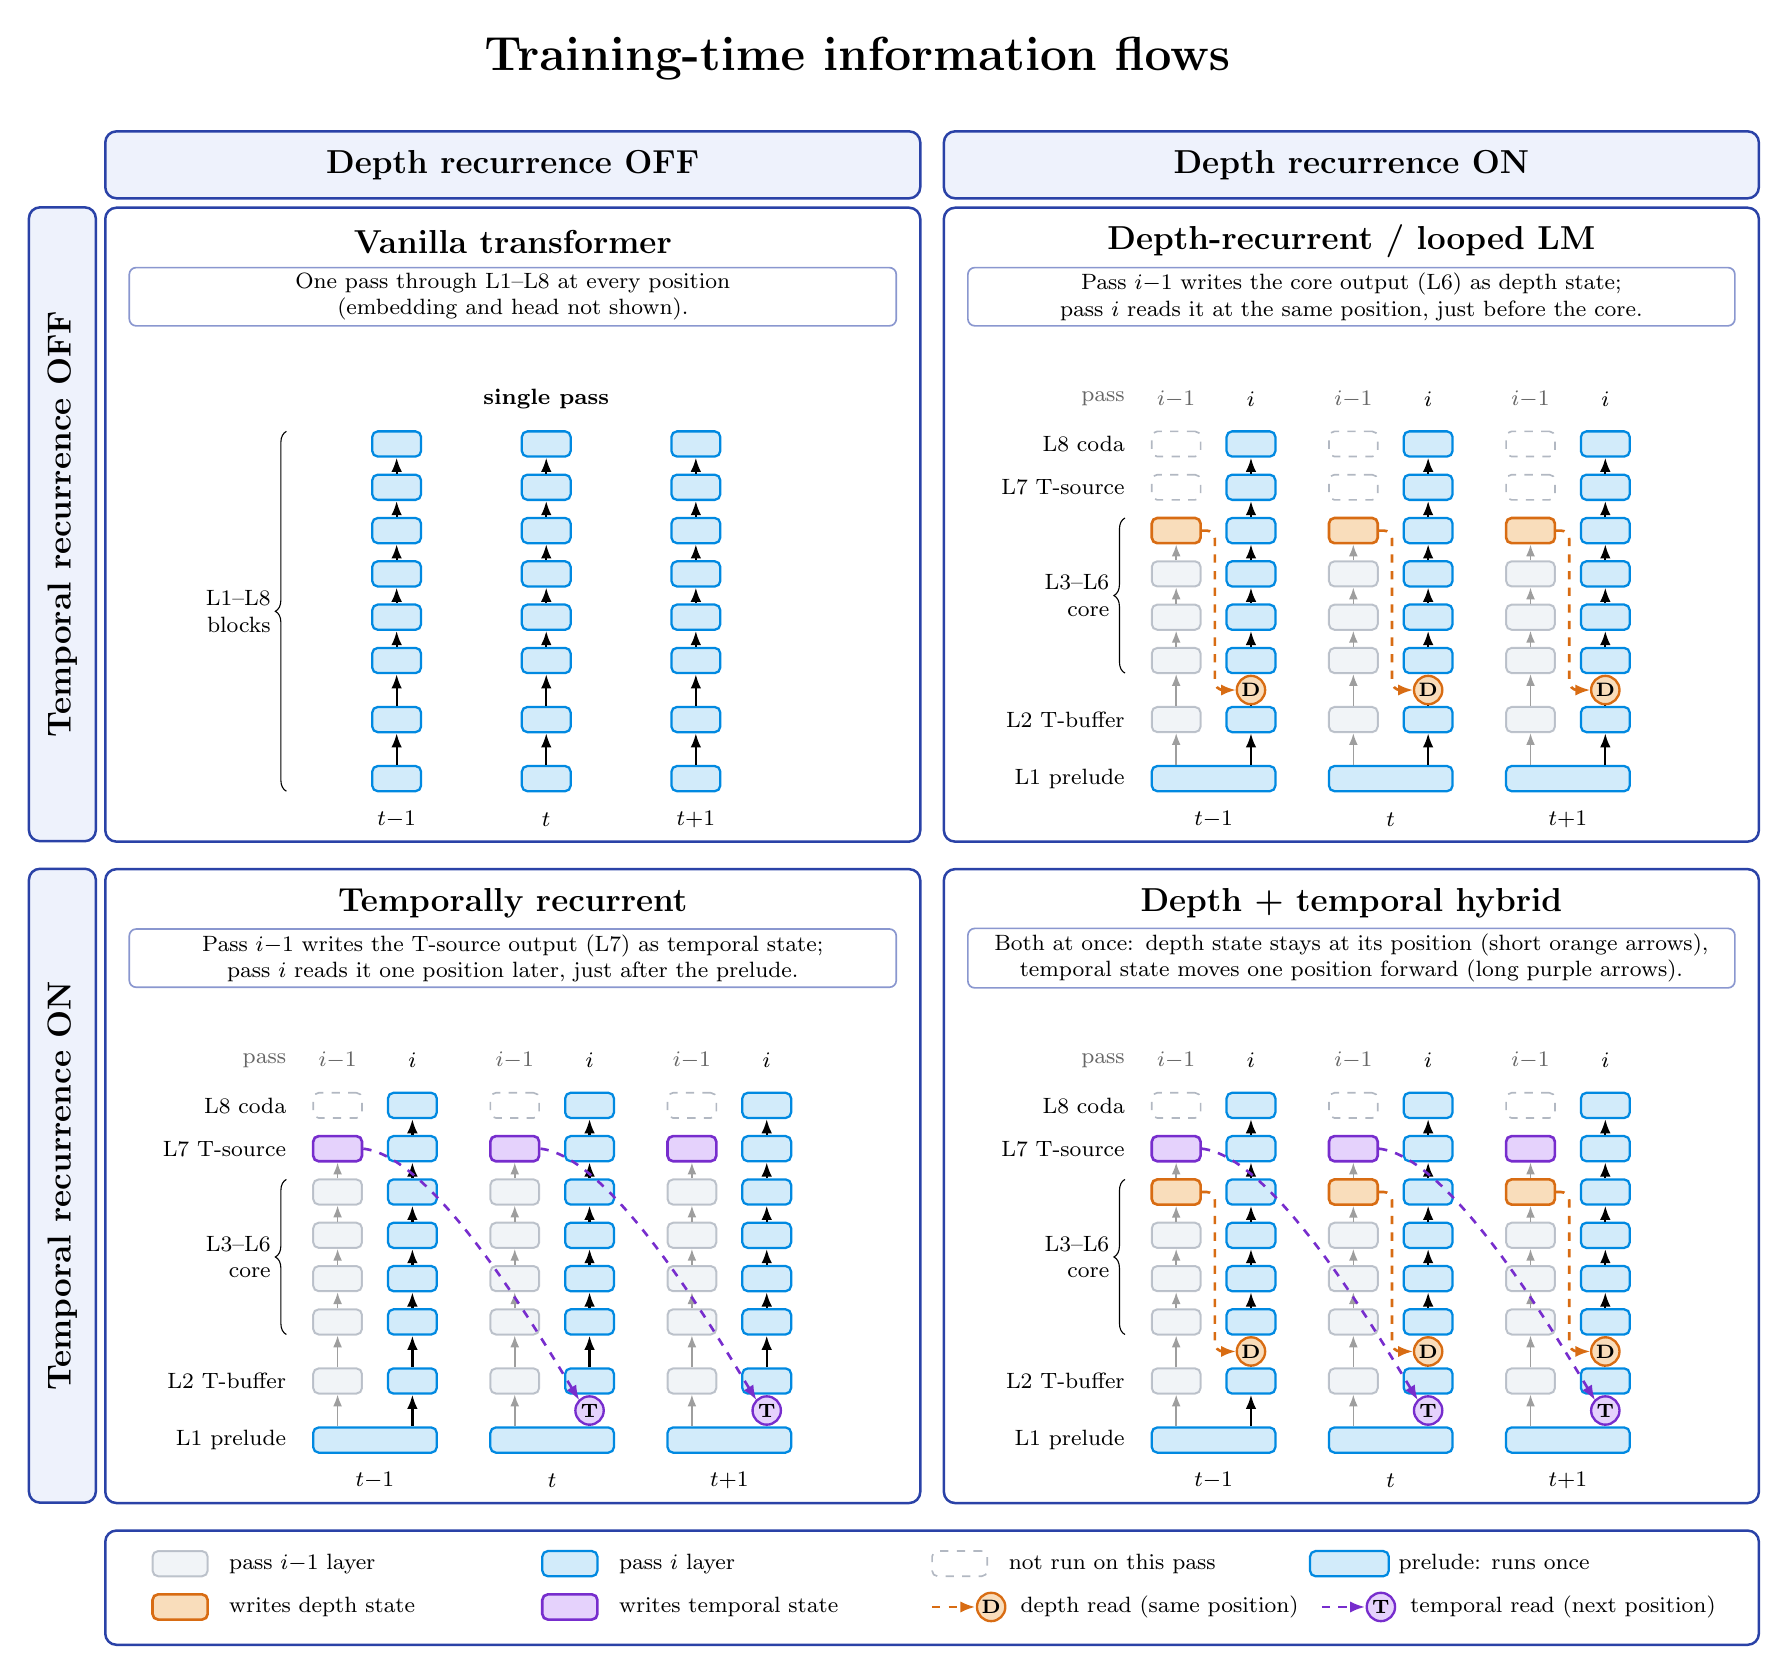
\begin{tikzpicture}[x=1cm,y=1cm]

\node[font=\bfseries\LARGE] at (11.9,17.30) {Training-time information flows};
\node[header, minimum width=10.35cm, minimum height=0.85cm, font=\bfseries\large] at (7.525,15.945) {Depth recurrence OFF};
\node[header, minimum width=10.35cm, minimum height=0.85cm, font=\bfseries\large] at (18.175,15.945) {Depth recurrence ON};
\node[sideheader, minimum width=8.05cm, minimum height=0.85cm, rotate=90, font=\bfseries\large] at (1.805,11.38) {Temporal recurrence OFF};
\node[sideheader, minimum width=8.05cm, minimum height=0.85cm, rotate=90, font=\bfseries\large] at (1.805,2.98) {Temporal recurrence ON};

% ---------------- Vanilla transformer
\begin{scope}[shift={(2.35,7.35)}]
  \draw[panel] (0,0) rectangle (10.35,8.05);
  \node[font=\bfseries\large] at (5.175,7.62) {Vanilla transformer};
  \node[descbox, text width=9.6cm] at (5.175,6.92) {One pass through L1--L8 at every position (embedding and head not shown).};
  \draw[decorate,decoration={brace,amplitude=4pt}] (2.3,0.64) -- (2.3,5.21) node[brace label] {L1--L8\\blocks};
  \node[font=\bfseries\footnotesize] at (5.60,5.62) {single pass};
  \node[active] (tlc0r1) at (3.700,0.800) {};
  \node[active] (tlc0r2) at (3.700,1.550) {};
  \node[active] (tlc0r3) at (3.700,2.300) {};
  \node[active] (tlc0r4) at (3.700,2.850) {};
  \node[active] (tlc0r5) at (3.700,3.400) {};
  \node[active] (tlc0r6) at (3.700,3.950) {};
  \node[active] (tlc0r7) at (3.700,4.500) {};
  \node[active] (tlc0r8) at (3.700,5.050) {};
  \draw[flow] (tlc0r1.north) -- (tlc0r2.south);
  \draw[flow] (tlc0r2.north) -- (tlc0r3.south);
  \draw[flow] (tlc0r3.north) -- (tlc0r4.south);
  \draw[flow] (tlc0r4.north) -- (tlc0r5.south);
  \draw[flow] (tlc0r5.north) -- (tlc0r6.south);
  \draw[flow] (tlc0r6.north) -- (tlc0r7.south);
  \draw[flow] (tlc0r7.north) -- (tlc0r8.south);
  \node[font=\footnotesize] at (3.7,0.28) {$t{-}1$};
  \node[active] (tlc1r1) at (5.600,0.800) {};
  \node[active] (tlc1r2) at (5.600,1.550) {};
  \node[active] (tlc1r3) at (5.600,2.300) {};
  \node[active] (tlc1r4) at (5.600,2.850) {};
  \node[active] (tlc1r5) at (5.600,3.400) {};
  \node[active] (tlc1r6) at (5.600,3.950) {};
  \node[active] (tlc1r7) at (5.600,4.500) {};
  \node[active] (tlc1r8) at (5.600,5.050) {};
  \draw[flow] (tlc1r1.north) -- (tlc1r2.south);
  \draw[flow] (tlc1r2.north) -- (tlc1r3.south);
  \draw[flow] (tlc1r3.north) -- (tlc1r4.south);
  \draw[flow] (tlc1r4.north) -- (tlc1r5.south);
  \draw[flow] (tlc1r5.north) -- (tlc1r6.south);
  \draw[flow] (tlc1r6.north) -- (tlc1r7.south);
  \draw[flow] (tlc1r7.north) -- (tlc1r8.south);
  \node[font=\footnotesize] at (5.6,0.28) {$t$};
  \node[active] (tlc2r1) at (7.500,0.800) {};
  \node[active] (tlc2r2) at (7.500,1.550) {};
  \node[active] (tlc2r3) at (7.500,2.300) {};
  \node[active] (tlc2r4) at (7.500,2.850) {};
  \node[active] (tlc2r5) at (7.500,3.400) {};
  \node[active] (tlc2r6) at (7.500,3.950) {};
  \node[active] (tlc2r7) at (7.500,4.500) {};
  \node[active] (tlc2r8) at (7.500,5.050) {};
  \draw[flow] (tlc2r1.north) -- (tlc2r2.south);
  \draw[flow] (tlc2r2.north) -- (tlc2r3.south);
  \draw[flow] (tlc2r3.north) -- (tlc2r4.south);
  \draw[flow] (tlc2r4.north) -- (tlc2r5.south);
  \draw[flow] (tlc2r5.north) -- (tlc2r6.south);
  \draw[flow] (tlc2r6.north) -- (tlc2r7.south);
  \draw[flow] (tlc2r7.north) -- (tlc2r8.south);
  \node[font=\footnotesize] at (7.5,0.28) {$t{+}1$};
\end{scope}

% ---------------- Depth-recurrent / looped LM
\begin{scope}[shift={(13.0,7.35)}]
  \draw[panel] (0,0) rectangle (10.35,8.05);
  \node[font=\bfseries\large] at (5.175,7.62) {Depth-recurrent / looped LM};
  \node[descbox, text width=9.6cm] at (5.175,6.92) {Pass $i{-}1$ writes the core output (L6) as depth state; pass $i$ reads it at the same position, just before the core.};
  \node[anchor=east, font=\footnotesize] at (2.42,0.8) {L1 prelude};
  \node[anchor=east, font=\footnotesize] at (2.42,1.55) {L2 T-buffer};
  \node[anchor=east, font=\footnotesize] at (2.42,4.5) {L7 T-source};
  \node[anchor=east, font=\footnotesize] at (2.42,5.05) {L8 coda};
  \draw[decorate,decoration={brace,amplitude=4pt}] (2.3,2.1399999999999997) -- (2.3,4.11) node[brace label] {L3--L6\\core};
  \node[anchor=east, font=\footnotesize, text=black!60] at (2.42,5.62) {pass};
  \node[font=\footnotesize, text=black!60] at (2.95,5.62) {$i{-}1$};
  \node[font=\bfseries\footnotesize] at (3.9000000000000004,5.62) {$i$};
  \node[active, minimum width=1.5699999999999998cm] (trpre0) at (3.425,0.800) {};
  \node[ghost] (trp0r2) at (2.950,1.550) {};
  \draw[ghostflow] (trpre0.north -| trp0r2) -- (trp0r2.south);
  \node[ghost] (trp0r3) at (2.950,2.300) {};
  \draw[ghostflow] (trp0r2.north) -- (trp0r3.south);
  \node[ghost] (trp0r4) at (2.950,2.850) {};
  \draw[ghostflow] (trp0r3.north) -- (trp0r4.south);
  \node[ghost] (trp0r5) at (2.950,3.400) {};
  \draw[ghostflow] (trp0r4.north) -- (trp0r5.south);
  \node[depthmark] (trp0r6) at (2.950,3.950) {};
  \draw[ghostflow] (trp0r5.north) -- (trp0r6.south);
  \node[notrun] (trp0r7) at (2.950,4.500) {};
  \node[notrun] (trp0r8) at (2.950,5.050) {};
  \node[active] (trq0r2) at (3.900,1.550) {};
  \node[active] (trq0r3) at (3.900,2.300) {};
  \node[active] (trq0r4) at (3.900,2.850) {};
  \node[active] (trq0r5) at (3.900,3.400) {};
  \node[active] (trq0r6) at (3.900,3.950) {};
  \node[active] (trq0r7) at (3.900,4.500) {};
  \node[active] (trq0r8) at (3.900,5.050) {};
  \draw[flow] (trpre0.north -| trq0r2) -- (trq0r2.south);
  \draw[flow] (trq0r2.north) -- (trq0r3.south);
  \draw[flow] (trq0r3.north) -- (trq0r4.south);
  \draw[flow] (trq0r4.north) -- (trq0r5.south);
  \draw[flow] (trq0r5.north) -- (trq0r6.south);
  \draw[flow] (trq0r6.north) -- (trq0r7.south);
  \draw[flow] (trq0r7.north) -- (trq0r8.south);
  \node[font=\footnotesize] at (3.4250000000000003,0.28) {$t{-}1$};
  \node[font=\footnotesize, text=black!60] at (5.2,5.62) {$i{-}1$};
  \node[font=\bfseries\footnotesize] at (6.15,5.62) {$i$};
  \node[active, minimum width=1.5699999999999998cm] (trpre1) at (5.675,0.800) {};
  \node[ghost] (trp1r2) at (5.200,1.550) {};
  \draw[ghostflow] (trpre1.north -| trp1r2) -- (trp1r2.south);
  \node[ghost] (trp1r3) at (5.200,2.300) {};
  \draw[ghostflow] (trp1r2.north) -- (trp1r3.south);
  \node[ghost] (trp1r4) at (5.200,2.850) {};
  \draw[ghostflow] (trp1r3.north) -- (trp1r4.south);
  \node[ghost] (trp1r5) at (5.200,3.400) {};
  \draw[ghostflow] (trp1r4.north) -- (trp1r5.south);
  \node[depthmark] (trp1r6) at (5.200,3.950) {};
  \draw[ghostflow] (trp1r5.north) -- (trp1r6.south);
  \node[notrun] (trp1r7) at (5.200,4.500) {};
  \node[notrun] (trp1r8) at (5.200,5.050) {};
  \node[active] (trq1r2) at (6.150,1.550) {};
  \node[active] (trq1r3) at (6.150,2.300) {};
  \node[active] (trq1r4) at (6.150,2.850) {};
  \node[active] (trq1r5) at (6.150,3.400) {};
  \node[active] (trq1r6) at (6.150,3.950) {};
  \node[active] (trq1r7) at (6.150,4.500) {};
  \node[active] (trq1r8) at (6.150,5.050) {};
  \draw[flow] (trpre1.north -| trq1r2) -- (trq1r2.south);
  \draw[flow] (trq1r2.north) -- (trq1r3.south);
  \draw[flow] (trq1r3.north) -- (trq1r4.south);
  \draw[flow] (trq1r4.north) -- (trq1r5.south);
  \draw[flow] (trq1r5.north) -- (trq1r6.south);
  \draw[flow] (trq1r6.north) -- (trq1r7.south);
  \draw[flow] (trq1r7.north) -- (trq1r8.south);
  \node[font=\footnotesize] at (5.675000000000001,0.28) {$t$};
  \node[font=\footnotesize, text=black!60] at (7.45,5.62) {$i{-}1$};
  \node[font=\bfseries\footnotesize] at (8.4,5.62) {$i$};
  \node[active, minimum width=1.5699999999999998cm] (trpre2) at (7.925,0.800) {};
  \node[ghost] (trp2r2) at (7.450,1.550) {};
  \draw[ghostflow] (trpre2.north -| trp2r2) -- (trp2r2.south);
  \node[ghost] (trp2r3) at (7.450,2.300) {};
  \draw[ghostflow] (trp2r2.north) -- (trp2r3.south);
  \node[ghost] (trp2r4) at (7.450,2.850) {};
  \draw[ghostflow] (trp2r3.north) -- (trp2r4.south);
  \node[ghost] (trp2r5) at (7.450,3.400) {};
  \draw[ghostflow] (trp2r4.north) -- (trp2r5.south);
  \node[depthmark] (trp2r6) at (7.450,3.950) {};
  \draw[ghostflow] (trp2r5.north) -- (trp2r6.south);
  \node[notrun] (trp2r7) at (7.450,4.500) {};
  \node[notrun] (trp2r8) at (7.450,5.050) {};
  \node[active] (trq2r2) at (8.400,1.550) {};
  \node[active] (trq2r3) at (8.400,2.300) {};
  \node[active] (trq2r4) at (8.400,2.850) {};
  \node[active] (trq2r5) at (8.400,3.400) {};
  \node[active] (trq2r6) at (8.400,3.950) {};
  \node[active] (trq2r7) at (8.400,4.500) {};
  \node[active] (trq2r8) at (8.400,5.050) {};
  \draw[flow] (trpre2.north -| trq2r2) -- (trq2r2.south);
  \draw[flow] (trq2r2.north) -- (trq2r3.south);
  \draw[flow] (trq2r3.north) -- (trq2r4.south);
  \draw[flow] (trq2r4.north) -- (trq2r5.south);
  \draw[flow] (trq2r5.north) -- (trq2r6.south);
  \draw[flow] (trq2r6.north) -- (trq2r7.south);
  \draw[flow] (trq2r7.north) -- (trq2r8.south);
  \node[font=\footnotesize] at (7.925000000000001,0.28) {$t{+}1$};
  \draw[dread, rounded corners=3pt] (trp0r6.east) -- ++(0.165,0) |- (3.710,1.925);
  \node[injectD] at (3.900,1.925) {D};
  \draw[dread, rounded corners=3pt] (trp1r6.east) -- ++(0.165,0) |- (5.960,1.925);
  \node[injectD] at (6.150,1.925) {D};
  \draw[dread, rounded corners=3pt] (trp2r6.east) -- ++(0.165,0) |- (8.210,1.925);
  \node[injectD] at (8.400,1.925) {D};
\end{scope}

% ---------------- Temporally recurrent
\begin{scope}[shift={(2.35,-1.05)}]
  \draw[panel] (0,0) rectangle (10.35,8.05);
  \node[font=\bfseries\large] at (5.175,7.62) {Temporally recurrent};
  \node[descbox, text width=9.6cm] at (5.175,6.92) {Pass $i{-}1$ writes the T-source output (L7) as temporal state; pass $i$ reads it one position later, just after the prelude.};
  \node[anchor=east, font=\footnotesize] at (2.42,0.8) {L1 prelude};
  \node[anchor=east, font=\footnotesize] at (2.42,1.55) {L2 T-buffer};
  \node[anchor=east, font=\footnotesize] at (2.42,4.5) {L7 T-source};
  \node[anchor=east, font=\footnotesize] at (2.42,5.05) {L8 coda};
  \draw[decorate,decoration={brace,amplitude=4pt}] (2.3,2.1399999999999997) -- (2.3,4.11) node[brace label] {L3--L6\\core};
  \node[anchor=east, font=\footnotesize, text=black!60] at (2.42,5.62) {pass};
  \node[font=\footnotesize, text=black!60] at (2.95,5.62) {$i{-}1$};
  \node[font=\bfseries\footnotesize] at (3.9000000000000004,5.62) {$i$};
  \node[active, minimum width=1.5699999999999998cm] (blpre0) at (3.425,0.800) {};
  \node[ghost] (blp0r2) at (2.950,1.550) {};
  \draw[ghostflow] (blpre0.north -| blp0r2) -- (blp0r2.south);
  \node[ghost] (blp0r3) at (2.950,2.300) {};
  \draw[ghostflow] (blp0r2.north) -- (blp0r3.south);
  \node[ghost] (blp0r4) at (2.950,2.850) {};
  \draw[ghostflow] (blp0r3.north) -- (blp0r4.south);
  \node[ghost] (blp0r5) at (2.950,3.400) {};
  \draw[ghostflow] (blp0r4.north) -- (blp0r5.south);
  \node[ghost] (blp0r6) at (2.950,3.950) {};
  \draw[ghostflow] (blp0r5.north) -- (blp0r6.south);
  \node[tempmark] (blp0r7) at (2.950,4.500) {};
  \draw[ghostflow] (blp0r6.north) -- (blp0r7.south);
  \node[notrun] (blp0r8) at (2.950,5.050) {};
  \node[active] (blq0r2) at (3.900,1.550) {};
  \node[active] (blq0r3) at (3.900,2.300) {};
  \node[active] (blq0r4) at (3.900,2.850) {};
  \node[active] (blq0r5) at (3.900,3.400) {};
  \node[active] (blq0r6) at (3.900,3.950) {};
  \node[active] (blq0r7) at (3.900,4.500) {};
  \node[active] (blq0r8) at (3.900,5.050) {};
  \draw[flow] (blpre0.north -| blq0r2) -- (blq0r2.south);
  \draw[flow] (blq0r2.north) -- (blq0r3.south);
  \draw[flow] (blq0r3.north) -- (blq0r4.south);
  \draw[flow] (blq0r4.north) -- (blq0r5.south);
  \draw[flow] (blq0r5.north) -- (blq0r6.south);
  \draw[flow] (blq0r6.north) -- (blq0r7.south);
  \draw[flow] (blq0r7.north) -- (blq0r8.south);
  \node[font=\footnotesize] at (3.4250000000000003,0.28) {$t{-}1$};
  \node[font=\footnotesize, text=black!60] at (5.2,5.62) {$i{-}1$};
  \node[font=\bfseries\footnotesize] at (6.15,5.62) {$i$};
  \node[active, minimum width=1.5699999999999998cm] (blpre1) at (5.675,0.800) {};
  \node[ghost] (blp1r2) at (5.200,1.550) {};
  \draw[ghostflow] (blpre1.north -| blp1r2) -- (blp1r2.south);
  \node[ghost] (blp1r3) at (5.200,2.300) {};
  \draw[ghostflow] (blp1r2.north) -- (blp1r3.south);
  \node[ghost] (blp1r4) at (5.200,2.850) {};
  \draw[ghostflow] (blp1r3.north) -- (blp1r4.south);
  \node[ghost] (blp1r5) at (5.200,3.400) {};
  \draw[ghostflow] (blp1r4.north) -- (blp1r5.south);
  \node[ghost] (blp1r6) at (5.200,3.950) {};
  \draw[ghostflow] (blp1r5.north) -- (blp1r6.south);
  \node[tempmark] (blp1r7) at (5.200,4.500) {};
  \draw[ghostflow] (blp1r6.north) -- (blp1r7.south);
  \node[notrun] (blp1r8) at (5.200,5.050) {};
  \node[active] (blq1r2) at (6.150,1.550) {};
  \node[active] (blq1r3) at (6.150,2.300) {};
  \node[active] (blq1r4) at (6.150,2.850) {};
  \node[active] (blq1r5) at (6.150,3.400) {};
  \node[active] (blq1r6) at (6.150,3.950) {};
  \node[active] (blq1r7) at (6.150,4.500) {};
  \node[active] (blq1r8) at (6.150,5.050) {};
  \draw[flow] (blpre1.north -| blq1r2) -- (blq1r2.south);
  \draw[flow] (blq1r2.north) -- (blq1r3.south);
  \draw[flow] (blq1r3.north) -- (blq1r4.south);
  \draw[flow] (blq1r4.north) -- (blq1r5.south);
  \draw[flow] (blq1r5.north) -- (blq1r6.south);
  \draw[flow] (blq1r6.north) -- (blq1r7.south);
  \draw[flow] (blq1r7.north) -- (blq1r8.south);
  \node[font=\footnotesize] at (5.675000000000001,0.28) {$t$};
  \node[font=\footnotesize, text=black!60] at (7.45,5.62) {$i{-}1$};
  \node[font=\bfseries\footnotesize] at (8.4,5.62) {$i$};
  \node[active, minimum width=1.5699999999999998cm] (blpre2) at (7.925,0.800) {};
  \node[ghost] (blp2r2) at (7.450,1.550) {};
  \draw[ghostflow] (blpre2.north -| blp2r2) -- (blp2r2.south);
  \node[ghost] (blp2r3) at (7.450,2.300) {};
  \draw[ghostflow] (blp2r2.north) -- (blp2r3.south);
  \node[ghost] (blp2r4) at (7.450,2.850) {};
  \draw[ghostflow] (blp2r3.north) -- (blp2r4.south);
  \node[ghost] (blp2r5) at (7.450,3.400) {};
  \draw[ghostflow] (blp2r4.north) -- (blp2r5.south);
  \node[ghost] (blp2r6) at (7.450,3.950) {};
  \draw[ghostflow] (blp2r5.north) -- (blp2r6.south);
  \node[tempmark] (blp2r7) at (7.450,4.500) {};
  \draw[ghostflow] (blp2r6.north) -- (blp2r7.south);
  \node[notrun] (blp2r8) at (7.450,5.050) {};
  \node[active] (blq2r2) at (8.400,1.550) {};
  \node[active] (blq2r3) at (8.400,2.300) {};
  \node[active] (blq2r4) at (8.400,2.850) {};
  \node[active] (blq2r5) at (8.400,3.400) {};
  \node[active] (blq2r6) at (8.400,3.950) {};
  \node[active] (blq2r7) at (8.400,4.500) {};
  \node[active] (blq2r8) at (8.400,5.050) {};
  \draw[flow] (blpre2.north -| blq2r2) -- (blq2r2.south);
  \draw[flow] (blq2r2.north) -- (blq2r3.south);
  \draw[flow] (blq2r3.north) -- (blq2r4.south);
  \draw[flow] (blq2r4.north) -- (blq2r5.south);
  \draw[flow] (blq2r5.north) -- (blq2r6.south);
  \draw[flow] (blq2r6.north) -- (blq2r7.south);
  \draw[flow] (blq2r7.north) -- (blq2r8.south);
  \node[font=\footnotesize] at (7.925000000000001,0.28) {$t{+}1$};
  \draw[tread] (blp0r7.east) .. controls +(0.9,-0.1) and +(-0.55,0.9) .. (6.020,1.305);
  \node[injectT] at (6.150,1.175) {T};
  \draw[tread] (blp1r7.east) .. controls +(0.9,-0.1) and +(-0.55,0.9) .. (8.270,1.305);
  \node[injectT] at (8.400,1.175) {T};
\end{scope}

% ---------------- Depth + temporal hybrid
\begin{scope}[shift={(13.0,-1.05)}]
  \draw[panel] (0,0) rectangle (10.35,8.05);
  \node[font=\bfseries\large] at (5.175,7.62) {Depth + temporal hybrid};
  \node[descbox, text width=9.6cm] at (5.175,6.92) {Both at once: depth state stays at its position (short orange arrows), temporal state moves one position forward (long purple arrows).};
  \node[anchor=east, font=\footnotesize] at (2.42,0.8) {L1 prelude};
  \node[anchor=east, font=\footnotesize] at (2.42,1.55) {L2 T-buffer};
  \node[anchor=east, font=\footnotesize] at (2.42,4.5) {L7 T-source};
  \node[anchor=east, font=\footnotesize] at (2.42,5.05) {L8 coda};
  \draw[decorate,decoration={brace,amplitude=4pt}] (2.3,2.1399999999999997) -- (2.3,4.11) node[brace label] {L3--L6\\core};
  \node[anchor=east, font=\footnotesize, text=black!60] at (2.42,5.62) {pass};
  \node[font=\footnotesize, text=black!60] at (2.95,5.62) {$i{-}1$};
  \node[font=\bfseries\footnotesize] at (3.9000000000000004,5.62) {$i$};
  \node[active, minimum width=1.5699999999999998cm] (brpre0) at (3.425,0.800) {};
  \node[ghost] (brp0r2) at (2.950,1.550) {};
  \draw[ghostflow] (brpre0.north -| brp0r2) -- (brp0r2.south);
  \node[ghost] (brp0r3) at (2.950,2.300) {};
  \draw[ghostflow] (brp0r2.north) -- (brp0r3.south);
  \node[ghost] (brp0r4) at (2.950,2.850) {};
  \draw[ghostflow] (brp0r3.north) -- (brp0r4.south);
  \node[ghost] (brp0r5) at (2.950,3.400) {};
  \draw[ghostflow] (brp0r4.north) -- (brp0r5.south);
  \node[depthmark] (brp0r6) at (2.950,3.950) {};
  \draw[ghostflow] (brp0r5.north) -- (brp0r6.south);
  \node[tempmark] (brp0r7) at (2.950,4.500) {};
  \draw[ghostflow] (brp0r6.north) -- (brp0r7.south);
  \node[notrun] (brp0r8) at (2.950,5.050) {};
  \node[active] (brq0r2) at (3.900,1.550) {};
  \node[active] (brq0r3) at (3.900,2.300) {};
  \node[active] (brq0r4) at (3.900,2.850) {};
  \node[active] (brq0r5) at (3.900,3.400) {};
  \node[active] (brq0r6) at (3.900,3.950) {};
  \node[active] (brq0r7) at (3.900,4.500) {};
  \node[active] (brq0r8) at (3.900,5.050) {};
  \draw[flow] (brpre0.north -| brq0r2) -- (brq0r2.south);
  \draw[flow] (brq0r2.north) -- (brq0r3.south);
  \draw[flow] (brq0r3.north) -- (brq0r4.south);
  \draw[flow] (brq0r4.north) -- (brq0r5.south);
  \draw[flow] (brq0r5.north) -- (brq0r6.south);
  \draw[flow] (brq0r6.north) -- (brq0r7.south);
  \draw[flow] (brq0r7.north) -- (brq0r8.south);
  \node[font=\footnotesize] at (3.4250000000000003,0.28) {$t{-}1$};
  \node[font=\footnotesize, text=black!60] at (5.2,5.62) {$i{-}1$};
  \node[font=\bfseries\footnotesize] at (6.15,5.62) {$i$};
  \node[active, minimum width=1.5699999999999998cm] (brpre1) at (5.675,0.800) {};
  \node[ghost] (brp1r2) at (5.200,1.550) {};
  \draw[ghostflow] (brpre1.north -| brp1r2) -- (brp1r2.south);
  \node[ghost] (brp1r3) at (5.200,2.300) {};
  \draw[ghostflow] (brp1r2.north) -- (brp1r3.south);
  \node[ghost] (brp1r4) at (5.200,2.850) {};
  \draw[ghostflow] (brp1r3.north) -- (brp1r4.south);
  \node[ghost] (brp1r5) at (5.200,3.400) {};
  \draw[ghostflow] (brp1r4.north) -- (brp1r5.south);
  \node[depthmark] (brp1r6) at (5.200,3.950) {};
  \draw[ghostflow] (brp1r5.north) -- (brp1r6.south);
  \node[tempmark] (brp1r7) at (5.200,4.500) {};
  \draw[ghostflow] (brp1r6.north) -- (brp1r7.south);
  \node[notrun] (brp1r8) at (5.200,5.050) {};
  \node[active] (brq1r2) at (6.150,1.550) {};
  \node[active] (brq1r3) at (6.150,2.300) {};
  \node[active] (brq1r4) at (6.150,2.850) {};
  \node[active] (brq1r5) at (6.150,3.400) {};
  \node[active] (brq1r6) at (6.150,3.950) {};
  \node[active] (brq1r7) at (6.150,4.500) {};
  \node[active] (brq1r8) at (6.150,5.050) {};
  \draw[flow] (brpre1.north -| brq1r2) -- (brq1r2.south);
  \draw[flow] (brq1r2.north) -- (brq1r3.south);
  \draw[flow] (brq1r3.north) -- (brq1r4.south);
  \draw[flow] (brq1r4.north) -- (brq1r5.south);
  \draw[flow] (brq1r5.north) -- (brq1r6.south);
  \draw[flow] (brq1r6.north) -- (brq1r7.south);
  \draw[flow] (brq1r7.north) -- (brq1r8.south);
  \node[font=\footnotesize] at (5.675000000000001,0.28) {$t$};
  \node[font=\footnotesize, text=black!60] at (7.45,5.62) {$i{-}1$};
  \node[font=\bfseries\footnotesize] at (8.4,5.62) {$i$};
  \node[active, minimum width=1.5699999999999998cm] (brpre2) at (7.925,0.800) {};
  \node[ghost] (brp2r2) at (7.450,1.550) {};
  \draw[ghostflow] (brpre2.north -| brp2r2) -- (brp2r2.south);
  \node[ghost] (brp2r3) at (7.450,2.300) {};
  \draw[ghostflow] (brp2r2.north) -- (brp2r3.south);
  \node[ghost] (brp2r4) at (7.450,2.850) {};
  \draw[ghostflow] (brp2r3.north) -- (brp2r4.south);
  \node[ghost] (brp2r5) at (7.450,3.400) {};
  \draw[ghostflow] (brp2r4.north) -- (brp2r5.south);
  \node[depthmark] (brp2r6) at (7.450,3.950) {};
  \draw[ghostflow] (brp2r5.north) -- (brp2r6.south);
  \node[tempmark] (brp2r7) at (7.450,4.500) {};
  \draw[ghostflow] (brp2r6.north) -- (brp2r7.south);
  \node[notrun] (brp2r8) at (7.450,5.050) {};
  \node[active] (brq2r2) at (8.400,1.550) {};
  \node[active] (brq2r3) at (8.400,2.300) {};
  \node[active] (brq2r4) at (8.400,2.850) {};
  \node[active] (brq2r5) at (8.400,3.400) {};
  \node[active] (brq2r6) at (8.400,3.950) {};
  \node[active] (brq2r7) at (8.400,4.500) {};
  \node[active] (brq2r8) at (8.400,5.050) {};
  \draw[flow] (brpre2.north -| brq2r2) -- (brq2r2.south);
  \draw[flow] (brq2r2.north) -- (brq2r3.south);
  \draw[flow] (brq2r3.north) -- (brq2r4.south);
  \draw[flow] (brq2r4.north) -- (brq2r5.south);
  \draw[flow] (brq2r5.north) -- (brq2r6.south);
  \draw[flow] (brq2r6.north) -- (brq2r7.south);
  \draw[flow] (brq2r7.north) -- (brq2r8.south);
  \node[font=\footnotesize] at (7.925000000000001,0.28) {$t{+}1$};
  \draw[dread, rounded corners=3pt] (brp0r6.east) -- ++(0.165,0) |- (3.710,1.925);
  \node[injectD] at (3.900,1.925) {D};
  \draw[dread, rounded corners=3pt] (brp1r6.east) -- ++(0.165,0) |- (5.960,1.925);
  \node[injectD] at (6.150,1.925) {D};
  \draw[tread] (brp0r7.east) .. controls +(0.9,-0.1) and +(-0.55,0.9) .. (6.020,1.305);
  \node[injectT] at (6.150,1.175) {T};
  \draw[dread, rounded corners=3pt] (brp2r6.east) -- ++(0.165,0) |- (8.210,1.925);
  \node[injectD] at (8.400,1.925) {D};
  \draw[tread] (brp1r7.east) .. controls +(0.9,-0.1) and +(-0.55,0.9) .. (8.270,1.305);
  \node[injectT] at (8.400,1.175) {T};
\end{scope}

% ---------------- Legend
\begin{scope}[shift={(2.35,-2.85)}]
  \draw[panel] (0,0) rectangle (21.00,1.45);
  \node[ghost, minimum width=0.70cm] at (0.95,1.03) {};
  \node[legendtext] at (1.45,1.03) {pass $i{-}1$ layer};
  \node[active, minimum width=0.70cm] at (5.90,1.03) {};
  \node[legendtext] at (6.40,1.03) {pass $i$ layer};
  \node[notrun, minimum width=0.70cm] at (10.85,1.03) {};
  \node[legendtext] at (11.35,1.03) {not run on this pass};
  \node[active, minimum width=1.0cm] at (15.80,1.03) {};
  \node[legendtext] at (16.30,1.03) {prelude: runs once};
  \node[depthmark, minimum width=0.70cm] at (0.95,0.48) {};
  \node[legendtext] at (1.45,0.48) {writes depth state};
  \node[tempmark, minimum width=0.70cm] at (5.90,0.48) {};
  \node[legendtext] at (6.40,0.48) {writes temporal state};
  \draw[dread] (10.50,0.48) -- (11.05,0.48);
  \node[injectD] at (11.25,0.48) {D};
  \node[legendtext] at (11.50,0.48) {depth read (same position)};
  \draw[tread] (15.45,0.48) -- (16.00,0.48);
  \node[injectT] at (16.20,0.48) {T};
  \node[legendtext] at (16.45,0.48) {temporal read (next position)};
\end{scope}
\end{tikzpicture}
\end{document}
